\section{Le Méta-Modèle Cinématique}
Le métamodèle cinématique est organisé autour de trois principaux packages:
\begin{itemize}
  \item \textbf{Toolkit}: représente les concepts liés à la définition des widgets\footnote{Elément visuel d'une interface graphique (bouton, ascenseur,liste déroulante, etc.)} \textsc{ihm}.
\newline
Le package Toolkit est construit de la manière suivante:
\newline
\begin{figure}[htb]
  \centering
  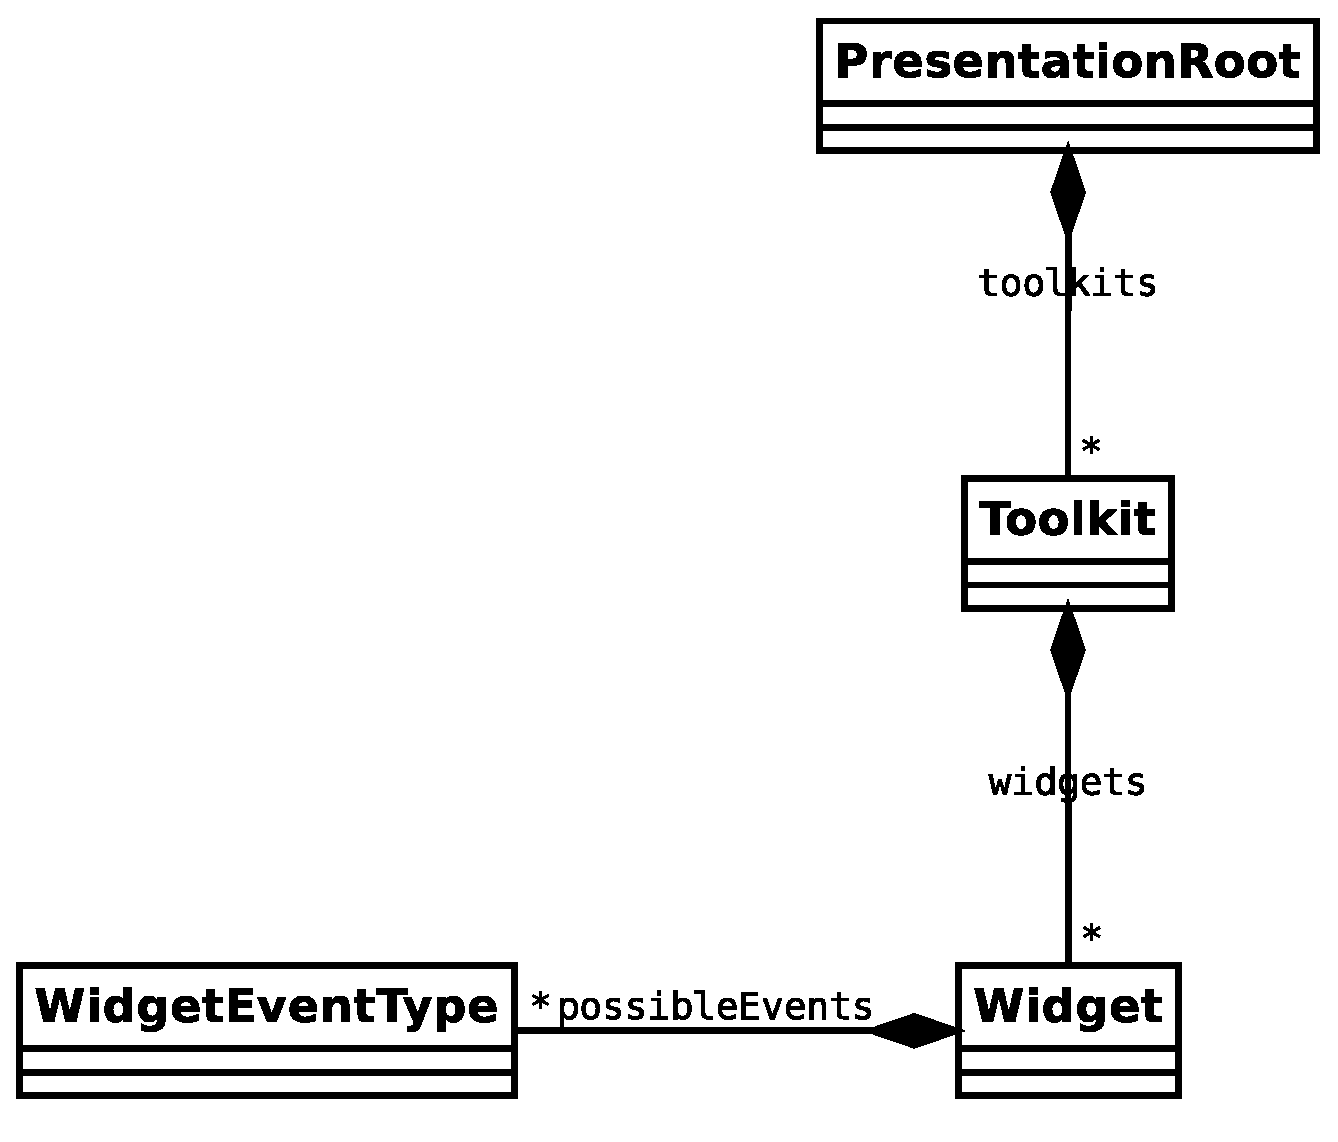
\includegraphics[scale=.3]{img/toolkit.eps}
  \caption{Métamodèle toolkit}
  \label{fig:Métamodèle Toolkit}
\end{figure}
  \item \textbf{View}: représente les concepts liés à la définition des écrans \textsc{ihm}.
\newline
Le package View est construit de la manière suivante:
\newline
\begin{figure}[H]
  \centering
  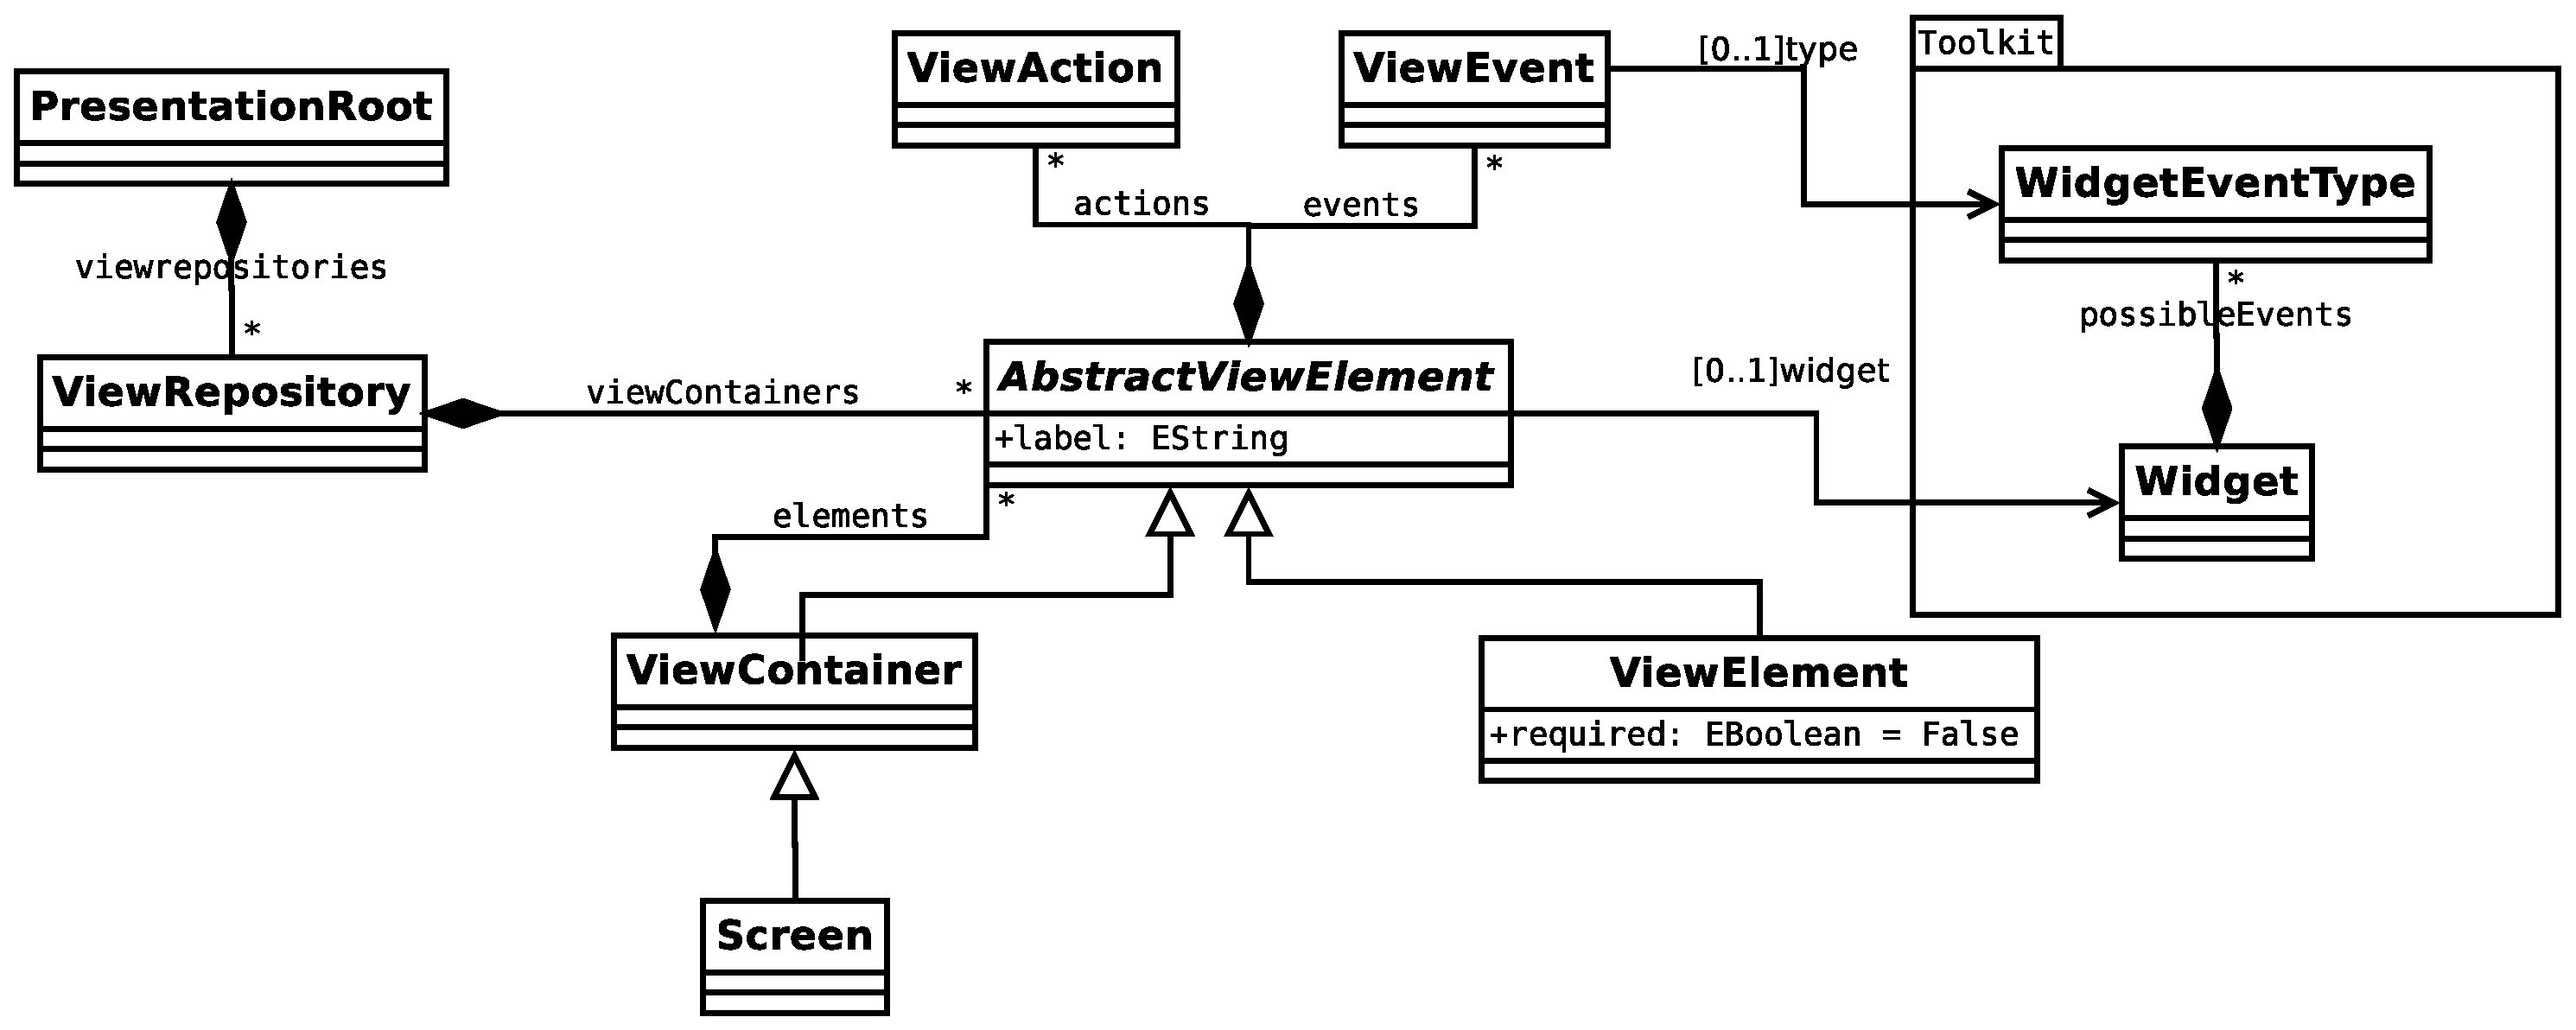
\includegraphics[scale=.3]{img/view.eps}
  \caption{Métamodèle view}
  \label{fig:Métamodèle View}
\end{figure}
  \item \textbf{Flow}: permet d'identifier le comportement dynamique des écrans \textsc{ihm}. Le flow peut être appréhendé comme une sorte de diagramme d'activités.
\newline
Le package Flow est construit de la manière suivante:
\newline
\begin{figure}[H]
  \centering
  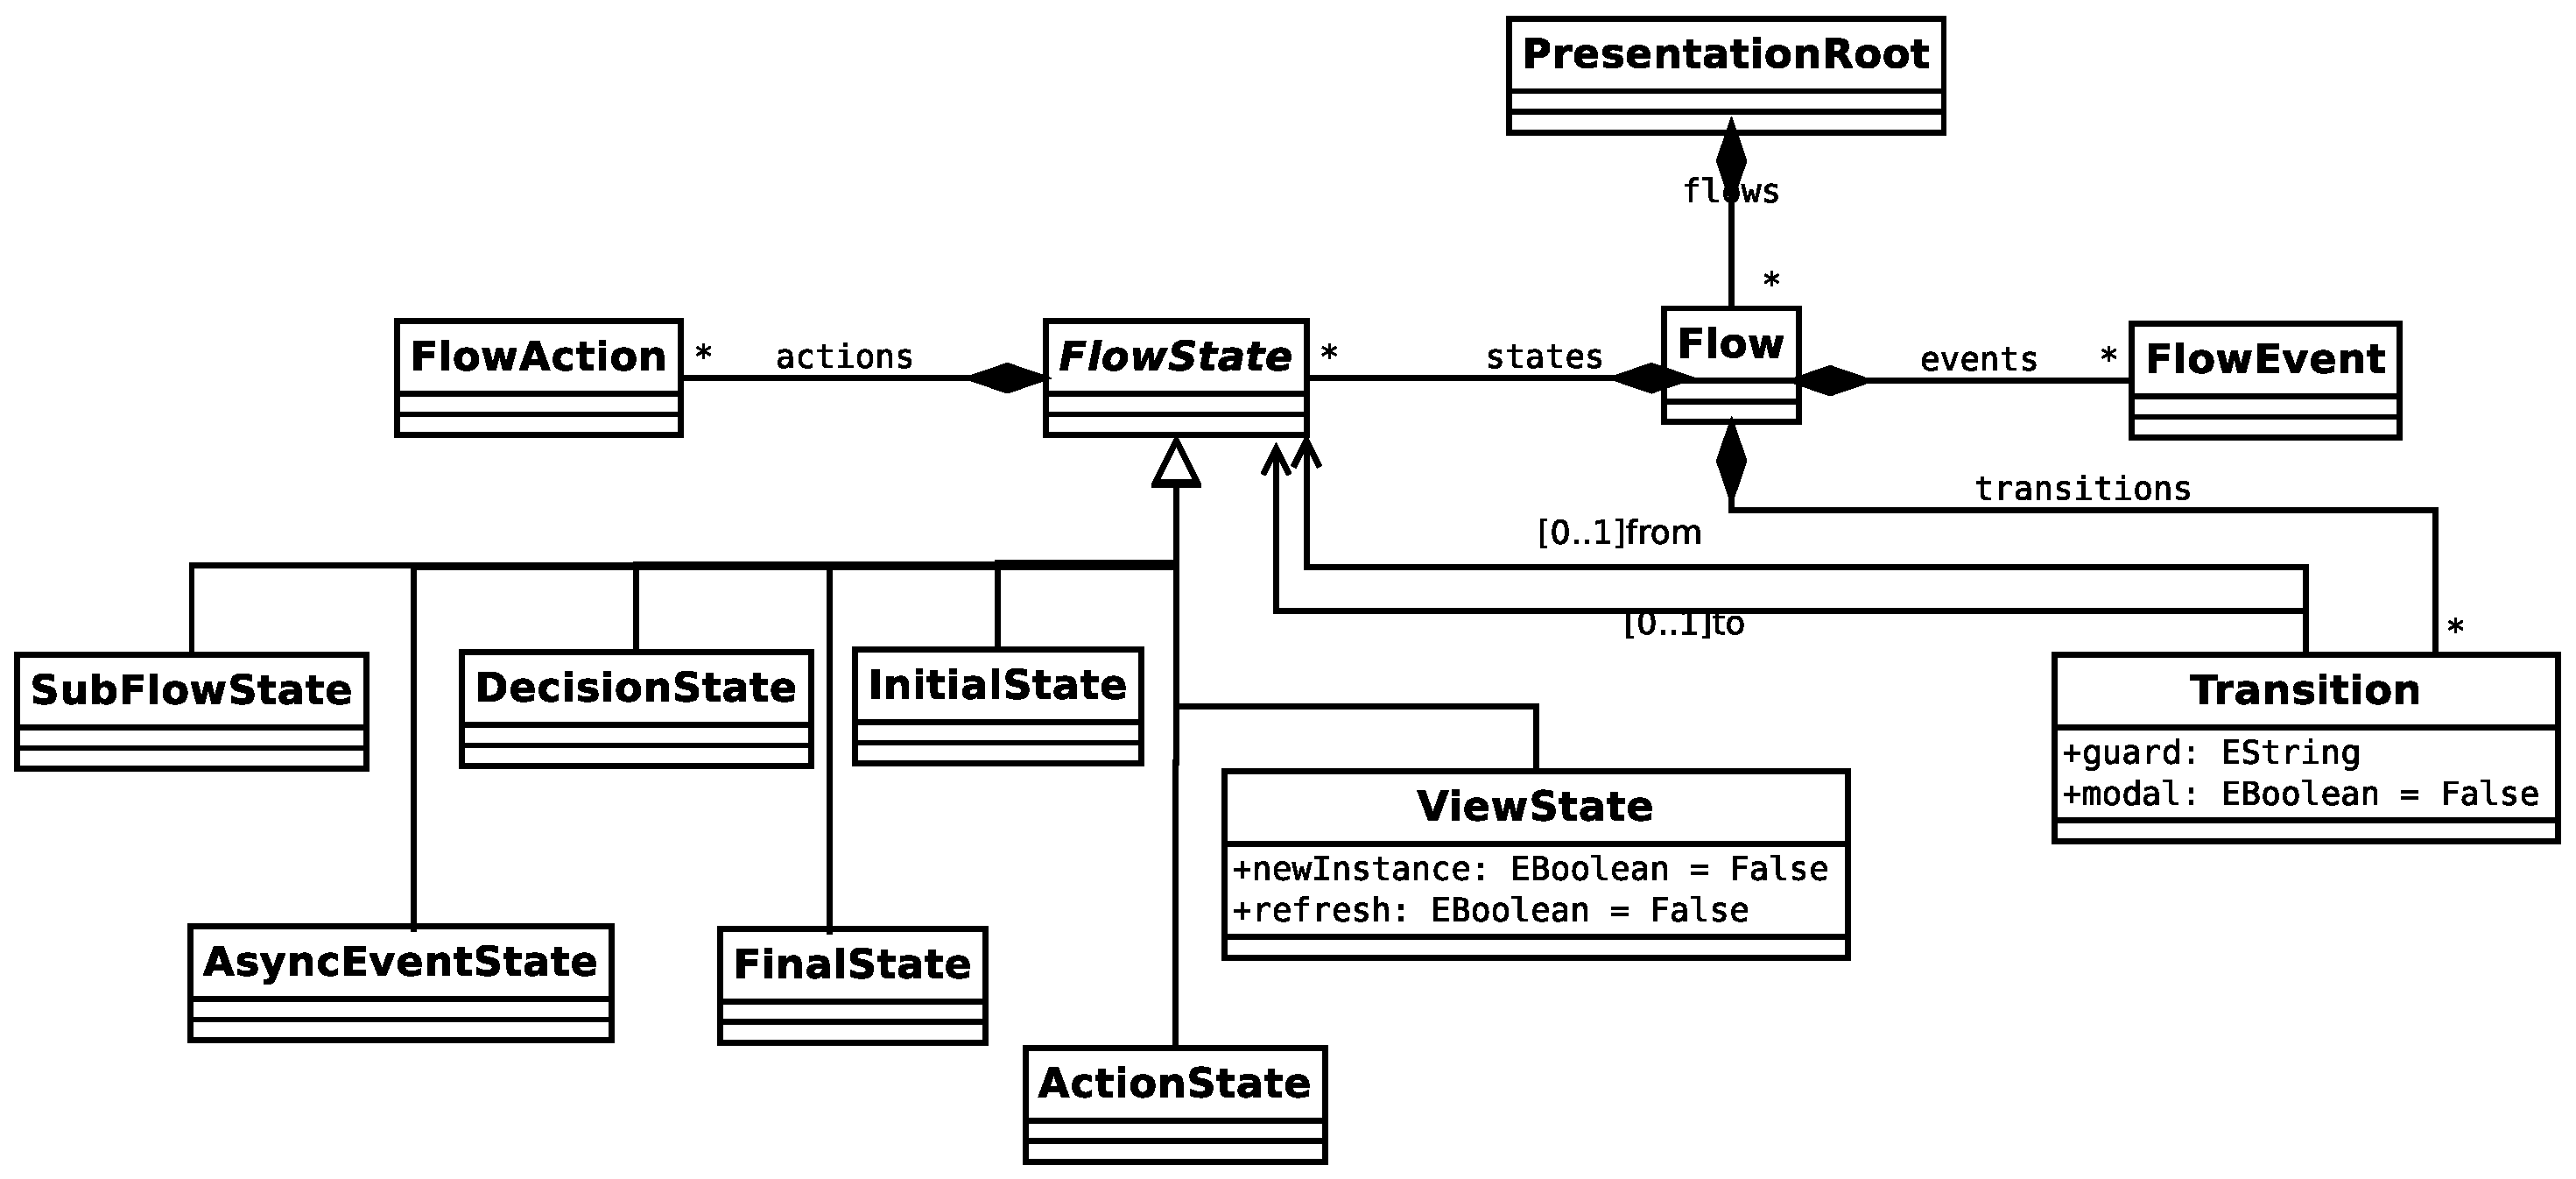
\includegraphics[scale=.3]{img/flow.eps}
  \caption{Métamodèle flow}
  \label{fig:Métamodèle Flow}
\end{figure}
\end{itemize}
\subsection{Le concept cinématique dans \kwplay{}}
Nous retrouvons dans \kwplay{} un repertoire dans lequel sont regroupés les différents fichiers Web (HTML, XML, …) liés aux vues (principe MVC). Les fichiers relatifs à la création des \textsc{ihm} sont donc indépendants du reste de l'application.   
\subsection{Conception du modèle}
La modélisation \textsc{ihm} de l'application prototype \texttt{Play} a été mise en place à l'aide de l'outil acceleo de \texttt{ObeoDesigner}. Le modèle est construit autour des trois principes du métamodèle défini précédemment:
\begin{enumerate}
\item \textbf{Toolkit}: Représente une palette contenant des widgets. Nous avons utilisé le modèle toolkit (par défaut) car il couvre tous les éléments de type "widget web" qui puissent exister (bouton, liste déroulante, champs de saisie, tableau, etc.). Chaque élément "widget" peut lever des événements de type \textit{WidgetEventType}.
\item \textbf{View} : Permet de représenter tous les éléments graphiques d'une interface utilisateur. Au plus haut niveau, nous définissons les éléments de type \textit{View Container}. 
\newline
Un \textit{View Container} peut être de type \textit{Page}, \textit{Panel} ou \textit{Table}. 
\newline
Nous choisissons le type \textit{Page} pour représenter un écran \textsc{ihm}. Ensuite, pour chaque ViewContainer, nous définissons les éléments qu'il contient, ça peut être un formulaire ou un tableau tout simplement. Nous construisons donc nos écrans, de cette manière, au fur et à mesure jusqu'à obtenir toutes les fenêtres \textsc{ihm} qui composent l'application.
\begin{figure}[H]
  \centering
  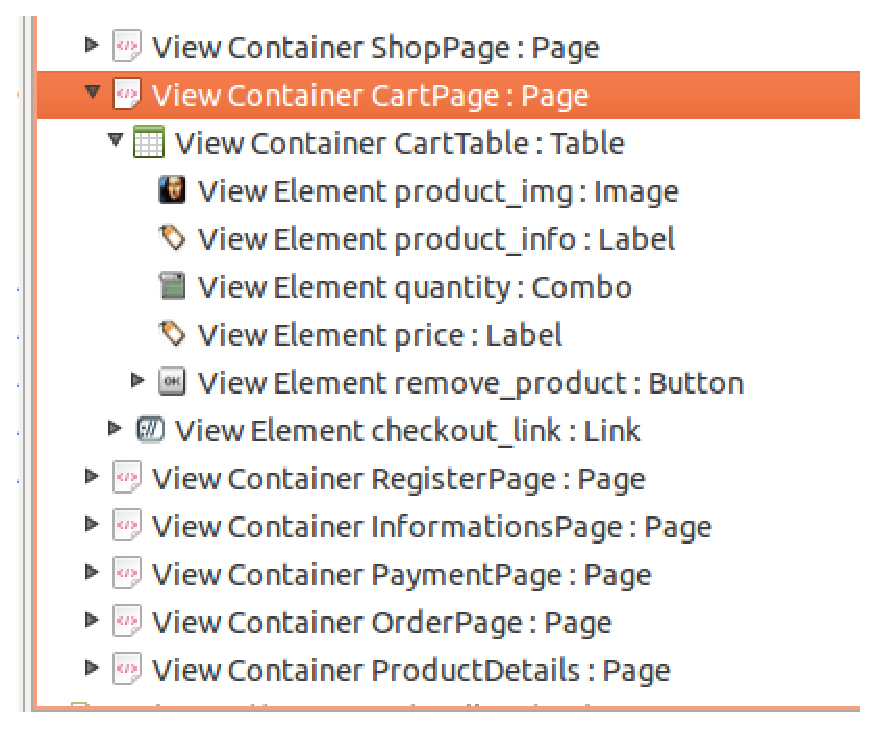
\includegraphics[scale=.4]{img/views.eps}
  \caption{Construction du modèle (partie Views)}
  \label{fig:Construction du modèle (partie Views)}
\end{figure}
\item \textbf{Flow} : Représente la manière dont les écrans de l'application peuvent s'enchaîner. Il décrit le comportement dynamique de l'\textsc{ihm} sous la forme d'enchaînements entre des états. Nous définissons ici, un état initial \textit{Initial State Start}, des états \textit{View State}, des états d'action \textit{Action State} et des transitions :
\begin{itemize}
\item Les états \textit{View State} correspondent aux écrans \textsc{ihm} et contiennent les \textit{View Container} décrit précédemment.
\item Les états d'action \textit{Action State} définissent les actions à réaliser sur chaque écran de l'application. Ils sont en liés aux fonctions offertes par la partie \kwsoa{}. 
\newline
\textit{Exemple}: Pour le chargement de la liste des produits disponibles pour la page d'acceuil (vitrine), nous définissons un \textit{Action State} nommé "Load Public Product List" que nous lions à l'opération getProductList() offerte par \kwsoa{}.  
\item Les transitions "\textit{Transition}" font passer l'\textsc{ihm} d'un état à un autre (d'un écran à un autre). 
\newline
\textit{Exemple}: Une transition pour l'affichage de l'écran d'acceuil "Display Main Page" va de l'état "Action State Load Public Product List" à l'état "View State Display MainPage".
\newline
Les transitions peuvent également avoir des conditions de garde.
\end{itemize}
\end{enumerate}				
\subsection{Génération du code}
Dans cette partie, nous nous occupons de générer les fichiers relatifs aux "routes", aux "controllers" et les "views". Rappelons les caractéristiques de chaque type de fichier:
\begin{itemize}
\item \textbf{Controller}: Nous avons une classe "MainController" dans laquelle nous déclarons des méthodes statiques pour chacune de nos Actions;
\item \textbf{Route}: Fichier de configuration des routes au sein de l'application. Les "routes" sont toutes associées au même controlleur "MainController".
\item \textbf{View}: Ensemble de fichiers décrivant un moteur de templates qui repose entièrement sur Scala ainsi que du code html pour la définition des formulaires, widgets, etc. 
\end{itemize}
BLABLABLABLA....
\subsection{Résultats obtenus}
BLABLABLABLA....
